\documentclass[12pt]{article}

\usepackage[shortlabels]{enumitem}
\usepackage{amsmath}
\usepackage{graphicx}

\title{Feedforward Control Homework 1}
\date{2019-03-10}
\author{Chien-Ming Chen, Na}

\begin{document}
  \maketitle
  \pagenumbering{arabic}

  \section{Problem 1}
  Consider the model of the flexural stage (Eq. (2) in the attachment by Hector Perez)

  \begin{enumerate}[(a)]
    \item What is the relative degree of the system?

    By definition,

    \begin{equation}
      \text{relative degree} = \text{order of denominator} – \text{order of numerator}
    \end{equation}

    In this case, the transfer function:

    \begin{equation}
      \text{TF} = \frac{11.88 s^4 + 4.977 s^3 + 539.6 s^2 + 129.9 s + 5625}{s^6 + 1.169 s^5 + 50.3 s^4 + 45.94 s^3 + 685.3 s^2 + 391.7 s + 1952}
    \end{equation}

    Where

    \begin{align*}
      \text{order of denominator} &= 6 \\
      \text{order of numerator} &= 4 \\
      \text{relative degree} &= 6 - 4 = 2
    \end{align*}

    \clearpage

    \item Find a state-space model (in control canonical form shown below) of this flexural stage.

    \begin{align*}
      A &= \left(\begin{array}{cccccc} -1.17 & -50.3 & -45.9 & -685.0 & -392.0 & -1966.0\\ 1.0 & 0 & 0 & 0 & 0 & 0\\ 0 & 1.0 & 0 & 0 & 0 & 0\\ 0 & 0 & 1.0 & 0 & 0 & 0\\ 0 & 0 & 0 & 1.0 & 0 & 0\\ 0 & 0 & 0 & 0 & 1.0 & 0 \end{array}\right) \\[2ex]
      B &= \left(\begin{array}{c} 1.0\\ 0\\ 0\\ 0\\ 0\\ 0 \end{array}\right) \\[2ex]
      C &= \left(\begin{array}{cccccc} 0 & 11.9 & 4.98 & 540.0 & 130.0 & 5622.0 \end{array}\right)
    \end{align*}

    \clearpage

    \item Find the inverse system model.

    \begin{align}
      \begin{split}
      \dot{x}_\text{inv} &= A_\text{inv} x_\text{inv} + B_\text{inv} y^{(r)}_d \\
             &= [A - BK_y] x + [BB_y] y^{(r)}_d \\
             &= \left(\begin{array}{cccccc} -0.419 & -45.4 & -10.9 & -473.0 & -5.68\,{10}^{-14} & 0\\ 1.0 & 0 & 0 & 0 & 0 & 0\\ 0 & 1.0 & 0 & 0 & 0 & 0\\ 0 & 0 & 1.0 & 0 & 0 & 0\\ 0 & 0 & 0 & 1.0 & 0 & 0\\ 0 & 0 & 0 & 0 & 1.0 & 0 \end{array}\right) x + \left(\begin{array}{c} 0.0842\\ 0\\ 0\\ 0\\ 0\\ 0 \end{array}\right) y^{(r)}_d
      \end{split}
      \\[2ex]
      \begin{split}
      u_\text{inv} &= C_\text{inv} x_\text{inv} + D_\text{inv} y^{(r)}_d \\
             &= [-K_y] x + [B_y] y^{(r)}_d \\
             &= [\frac{-CA^r}{CA^{r-1}B}] x + [\frac{1}{CA^{r-1}B}] y^{(r)}_d \\
             &= \left(\begin{array}{cccccc} 0.75 & 4.88 & 35.0 & 212.0 & 392.0 & 1966.0 \end{array}\right) x + 0.0842\ y^{(r)}_d
      \end{split}
    \end{align}

    \clearpage

    \item Simulate the inverse system model using MATLAB(lsim command) to find the inverse feedforward input. The desired acceleration profile is shown below.
    \item Apply this feedforward input to the system model found in part (b) to verify that the output tracking of y is achieved (use lsim command again).

    \begin{figure}[h]
      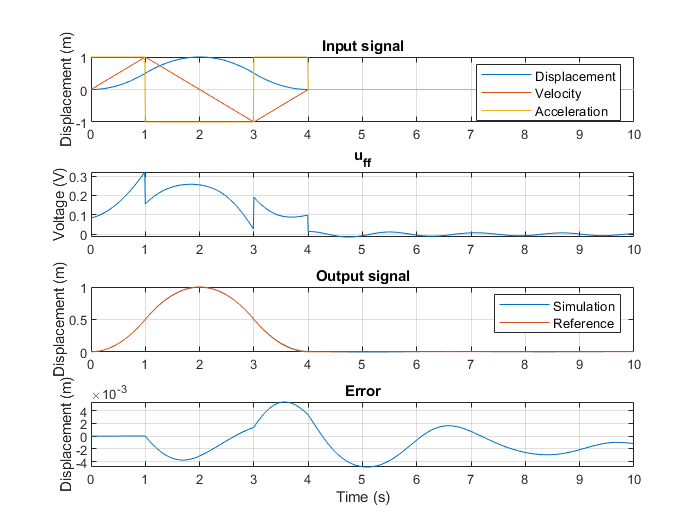
\includegraphics[width=15cm]{result_de}
      \caption{Simulation result}
      \centering
    \end{figure}

    \clearpage

    \item Investigate the effect of 5\% variation in the DC gain of the system; in particular simulate the response of the system (using the original inverse input) when the numerator constant 5625 has changed by 5\% and -5\%. What is the maximum error in the output? How could this error be reduced?

    \begin{figure}[h]
      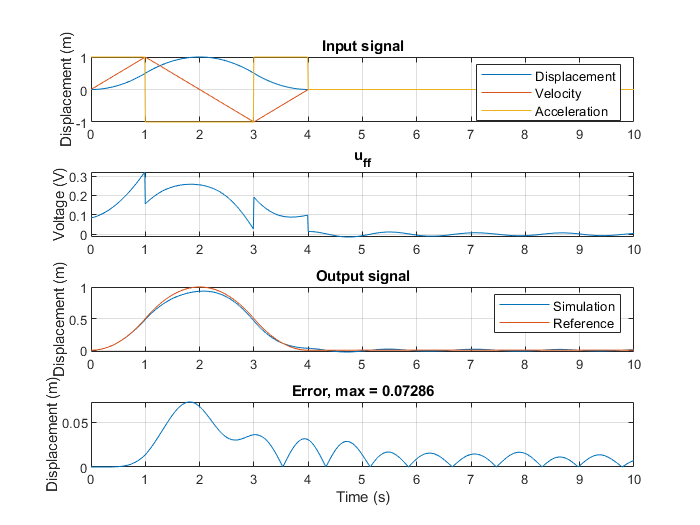
\includegraphics[width=15cm]{result_f_1}
      \caption{System changed by -5\%}
      \centering
    \end{figure}

    \begin{figure}[h]
      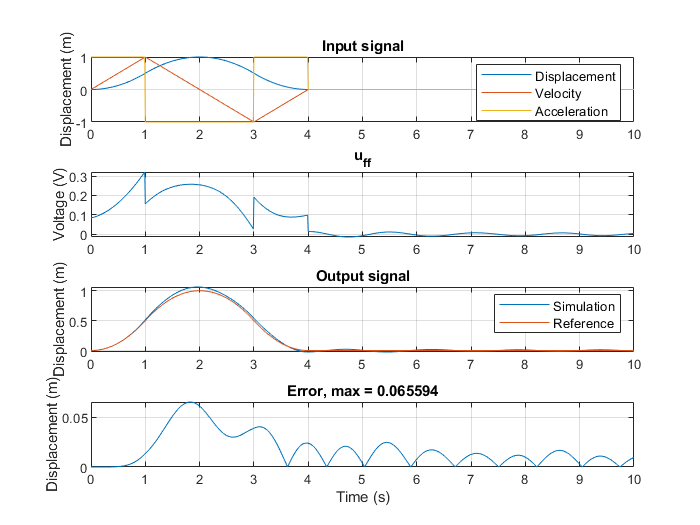
\includegraphics[width=15cm]{result_f_2}
      \caption{System changed by 5\%}
      \centering
    \end{figure}



  \end{enumerate}

\end{document}
